\documentclass[12pt]{article}
\usepackage[margin=1in]{geometry}
\usepackage{hyperref}
\usepackage{multicol}
\usepackage{upgreek}
\usepackage{graphicx}
\usepackage[section]{placeins} % Keeps images within their section. 
\usepackage{longtable}
\DeclareGraphicsExtensions{.pdf,.png,.jpg}

%perhaps comment this out later. 
\newcommand{\Sum}[3]{\sum_{#1}^{#2} #3}

\pdfinfo{%
  /Title    (Project1)
  /Author   (Clinton McKay)
  /Creator  (Clinton McKay)
  /Producer (Clinton McKay)
  /Subject  (CSCI 444 -- Data Visualization) 
  /Keywords (CSCI444)
}

\title{Final Project: Homicides\\{\Large My Visuals}}
\date{\today}
\author{Clinton McKay}

\begin{document}

\maketitle

\section{Overview}
As a first world country, is the United States a safer place to live than a third world country? Have we developed a false sense of security since there are no active warlike conflicts in this country? Is it true that developing countries are less "civilized" and that there exists higher violent crime rates? This analysis will delve into the science of info graphics to present a detailed yet simple explanation of what crime is like our world. 

\section{Hypothesis}
Homicide rates are not affected by the development status of the country. The categories are; Developed, developing, and transitioning.

\section{Data}
The primary datasource for the project will be the homicides data from the UN Statistics Database. The visualization of the choropleth was made possible due to the shape file created by {\em Bjorn Sandvik at thematicmapping.org}. The latest version of his shape file can be downloaded at http://thematicmapping.org/downloads/world\_borders.php. If the link is broken the shapefile can also be accessed from the {\em data/mapdata} folder. 

\section{Supporting Visuals}
For my supporting visuals I decided to use simple bipartite plots to show the distribution of homicide rates amongst the development categories of the countries. Since I was interested in the distribution of the homicide rates for the countries. I decided to create a box plot (figure \ref{fig:sub-box}) see what the distribution of the homicide rates was amongst the different countries. In addition to using a box plot a violin plot was used (figure \ref{fig:sup-violin}) to show the distribution of countries at various homicide rates. A violin plot is similar to a histogram the only difference is that it has been mirrored so that the shape is symmetric. Violin plots provide the advantage of allowing the user to compare distributions without too much mental effort. Figure \ref{fig:sup-line} is a simple time series plot of the homicide rates amongst the different country development states.  

\begin{figure}[!ht]
    \centering
    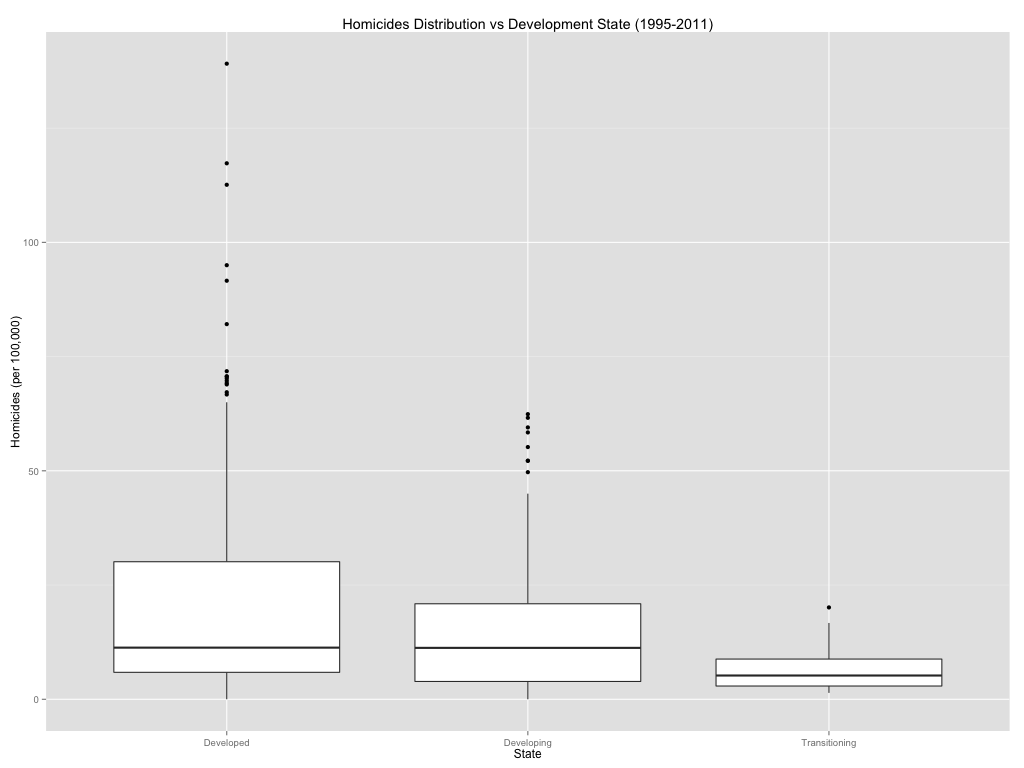
\includegraphics[width=7in, keepaspectratio]{supporting_visual_box.png}
    \caption{A box plot comparing the crime rates between 1995 - 1997 of the countries belonging to the following UN regions and categories: Latin America and the Caribbean, Northern America, Caribbean, Central America , South America, and Developing regions}
    \label{fig:sub-box}
\end{figure}

\begin{figure}[!ht]
    \centering
    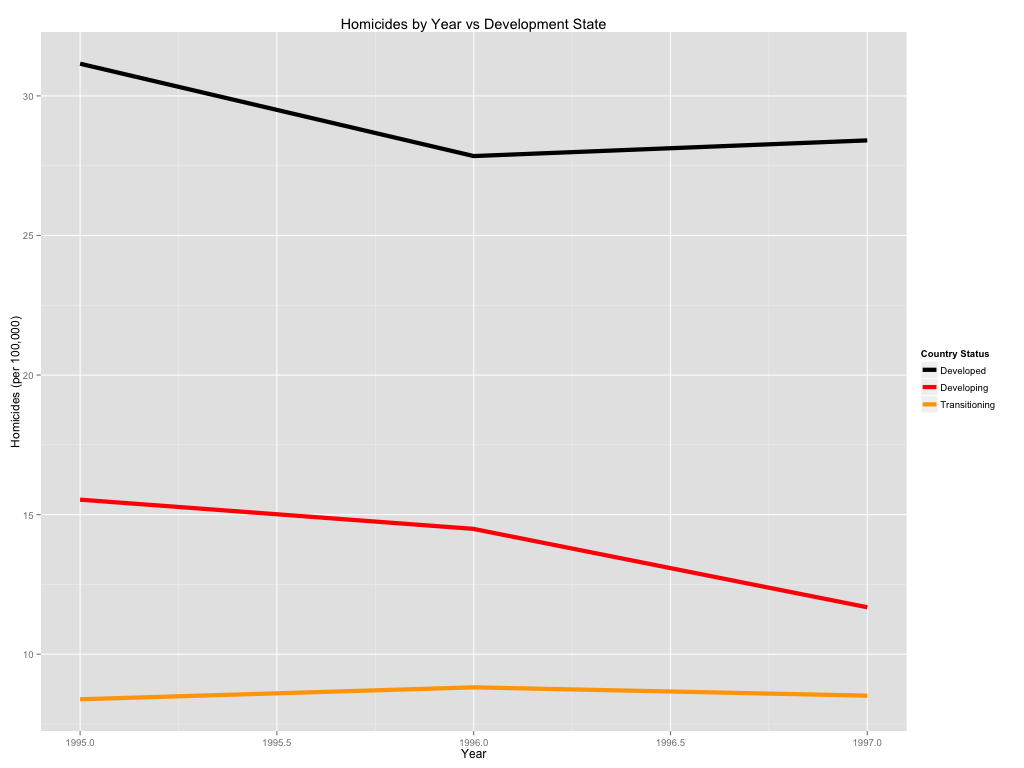
\includegraphics[width=7in, keepaspectratio]{supporting_visual_line.png}
    \caption{Comparison of the crime rates between 1995 - 1997 of the countries belonging to the following UN regions and categories: Latin America and the Caribbean, Northern America, Caribbean, Central America , South America, and Developing regions. Each line represents a category average.}
    \label{fig:sup-line}
\end{figure}

\begin{figure}[!ht]
    \centering
    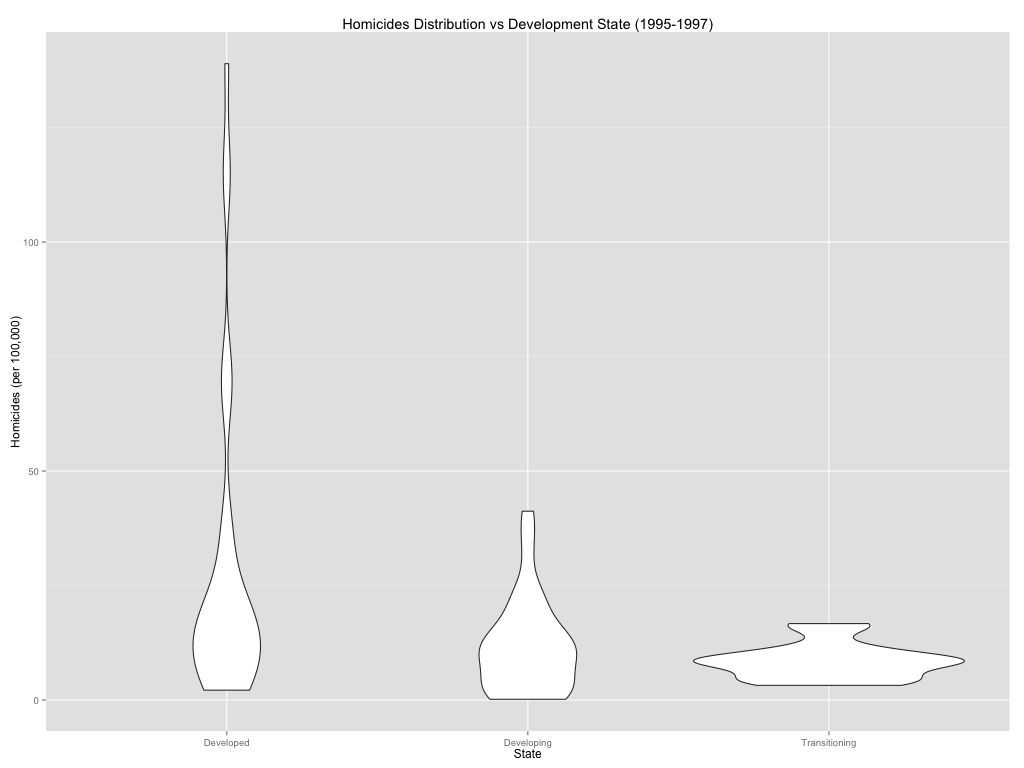
\includegraphics[width=7in, keepaspectratio]{supporting_visual_violin.png}
    \caption{A violin plot showing the distribution of crime rates between 1995-1997 for the countries in the following UN regions and categories: Latin America and the Caribbean, Northern America, Caribbean, Central America , South America, and Developing regions. Each line represents a category average.}
    \label{fig:sup-violin}
\end{figure}

\section{Refuting Visuals}
To refute the hypothesis a choropleth (figure \ref{fig:ref-choropleth}) that visualizes the homicide rates was used. This graph is a graph refuting visual because it quickly refutes the hypothesis without requiring too much interpretation. Applying a colored border to the countries allows quick discovery of the developed and developing nations. While at the same time they do not distract from the fill color of the country. 

\begin{figure}[!ht]
    \centering
    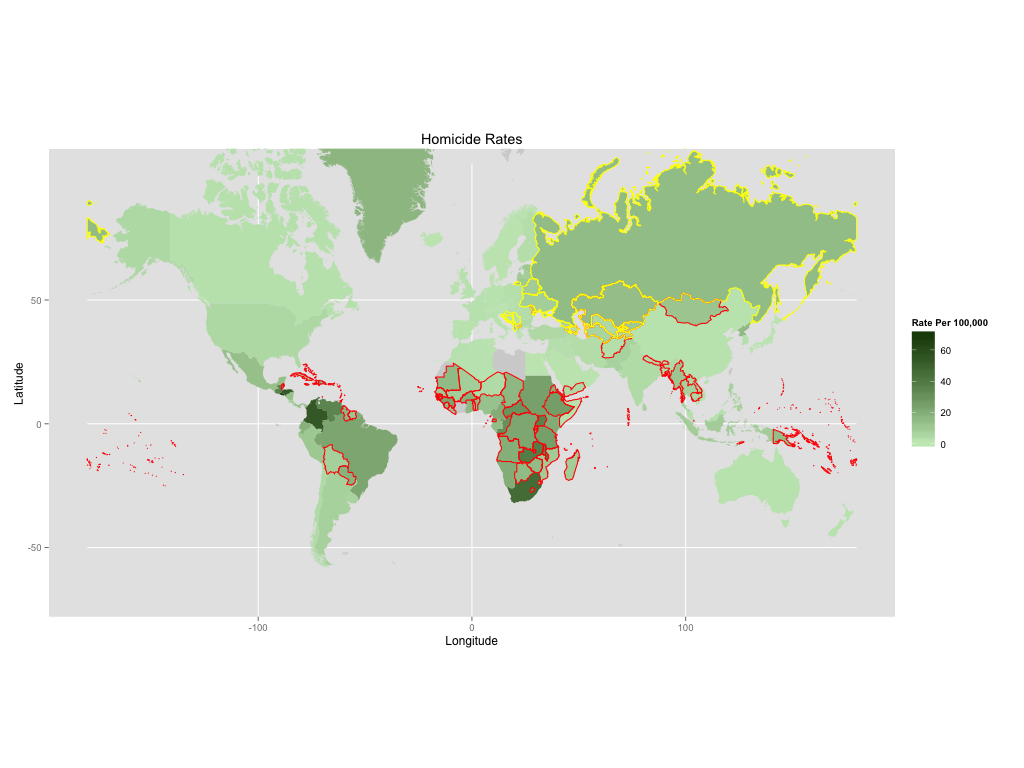
\includegraphics[width=7in, keepaspectratio]{refuting_world_hom_ave.png}
    \caption{Choropleth of the world. The fill color represents the rate (gray fill represents NA values) and the border color of the countries represents the development state of the countries. Red, yellow, and no borders represent developing, transitioning, and developed respectively. }
    \label{fig:ref-choropleth}
\end{figure}


%Figures \ref{fig:refreversestep} and \ref{fig:refrandom} refute my hypothesis. After shaking the balls, the degree distrubution for quartiles Q2 and Q3 actually increase. The reason for this behavior was due to particles clustering around bigger particles as the simulation was vibrating. 
%
%\begin{figure}[!ht]
%    \centering
%    \includegraphics[width=7in, keepaspectratio]{ReverseStepSeeding.png}
%    \caption{Plot showing the quartiles of the degree distribution of the balls after being seeded with a reverse step seed. Same as the step seed except particles are generated with radii in descending order from the maximum radius to the minimum radius.}
%    \label{fig:refreversestep}
%\end{figure}
%
%\begin{figure}[!ht]
%    \centering
%    \includegraphics[width=7in, keepaspectratio]{RandomSeeding.png}
%    \caption{Plot showing the quartiles of the degree distribution of the balls after being seeded with a random seed (randomly generated radii).}
%    \label{fig:refrandom}
%\end{figure}
%
%\section{Simulation Visuals}
%
%\begin{figure}[!ht]
%    \centering
%    \includegraphics[width=7in, keepaspectratio]{glStandard.png}
%    \caption{Standard view of the particles.}
%    \label{fig:glstandard}
%\end{figure}
%
%\begin{figure}[!ht]
%    \centering
%    \includegraphics[width=7in, keepaspectratio]{glForce.png}
%    \caption{Viewing the particles and their interacting forces.}
%    \label{fig:glforce}
%\end{figure}
%
%\begin{figure}[!ht]
%    \centering
%    \includegraphics[width=7in, keepaspectratio]{glForce_Vel.png}
%    \caption{Viewing the particles and their interacting forces and velocities.}
%    \label{fig:glforce_vel}
%\end{figure}

\end{document}
